\subsection{Till}
\paragraph{} This simulation's model represent the till. The customer does the bill and pays. This is included in service time. After this module the customer goes out of the system. 

\begin{figure}[h]
  \begin{center}
  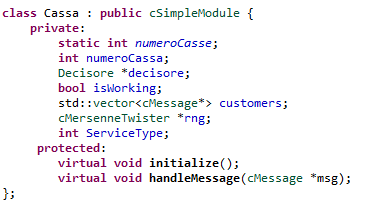
\includegraphics[width=80mm]{till.png}
  \caption{Till.}
  \label{fig:till}
  \end{center}
\end{figure}

\paragraph{initialize} This function will initialize all the port gates of Coda, because it need as many outputs ports as the number of Casse in the simulation. Then the simulation will start.

\paragraph{handleMessage} This function manage the queue: it check if a new customer is arrived, if there is at least one customer in the queue and there is at least one available till, it send the customer to the till.
